\section{SnapStart}\label{chapter:snapstart}

Jednym z istotnych czynników wpływających na wydajność funkcji AWS Lambda implementowanych w ekosystemie Java jest zjawisko tzw. zimnego startu.
Wynika on z cyklu życia funkcji i etapu inicjalizacji (co zostało opisane w Rozdziale \ref{chapter:aws_lambda}).
W etap ten wchodzą procesy takie jak inicjalizacja maszyny wirtualnej Java czy uruchomienie statycznego kodu inicjującego \cite{awsLambdaDocs}.
W przypadku Javy zajmuje to więcej czasu niż dla innych języków (jak Python), co wydłuża zimne starty \cite{8605773}.
Znacząco oddziałuje to na wydajność funkcji, a może być szczególnie dotkliwe dla serwisów o niewielkiej aktywności.
W odpowiedzi na potrzebę minimalizacji tych negatywnych skutków Amazon Web Services wprowadziło mechanizm znany jako AWS Lambda SnapStart.
W ramach podrozdziału podjęto analizę tego rozwiązania w kontekście jego działania, zalet oraz ograniczeń. 

Mechanizm SnapStart istotnie modyfikuje tradycyjny cykl życia funkcji AWS Lambda.
Zasadnicza różnica polega na przeniesieniu kosztownego etapu inicjalizacji z momentu pierwszego wywołania funkcji na etap jej publikacji \cite{amazonSnapstartDeveloperGUide}.
Oznacza to, że inicjalizacja funkcji nie jest wykonywana w momencie zapytania użytkownika (co wywołuje zimny start), lecz w momencie wgrania nowej wersji funkcji (oraz kodu) przez programistę.
Inicjalizacja ta zawiera najdłuższe operacje dla rozwiązań Java jak utworzenie maszyny wirtualnej, załadowanie klas, czy wykonanie kodu inicjalizującego.
Następnie, tworzona jest zaszyfrowana ,,migawka'' (ang. snapshot) stanu pamięci i dysku w pełni gotowego środowiska wykonawczego.
Gdy funkcja jest następnie wywoływana po raz pierwszy, nie zachodzi już standardowy zimny start.
Zamiast tego środowisko jest odtwarzane z utworzonej migawki, co zostało przedstawione na Rysunku \ref{fig:aws_lambda_snapstart_process}.
Według dostawcy AWS metoda ta w optymalnych scenariuszach zmniejsza opóźnienie z kilku sekund do mniej niż sekundy \cite{amazonSnapstartDeveloperGUide}. 

\begin{figure}[h]
    \centering
    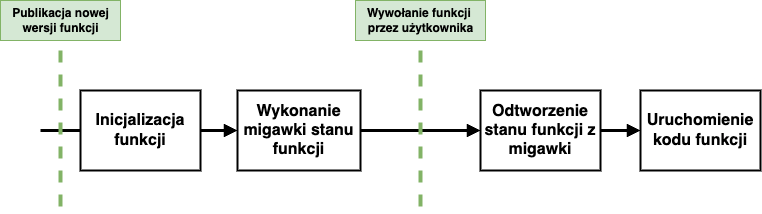
\includegraphics[width=0.95\textwidth]{charts/snapstart.png}
    \caption{Proces uruchomienia AWS Lambda z użyciem metody SnapStart [źródło:~opracowanie~własne]}
    \label{fig:aws_lambda_snapstart_process}
\end{figure}

Działanie tej metody jest technicznie możliwe dzięki użyciu środowiska wirtualizacji przez AWS Lambda.
Jak opisują Agache i inni autorzy \cite{246288} usługa Lambda do izolacji poszczególnych funkcji wykorzystuje dedykowane maszyny wirtualne typu microVM.
Są one zarządzane przez lekki monitor maszyn wirtualnych (ang. VMM) o nazwie Firecracker.
Posiada on cechy, które były kluczowe w minimalizacji problemu zimnego startu.
Po pierwsze, celowo rezygnuje on z emulacji zbędnych urządzeń (jak emulacja systemu BIOS czy rozbudowanych kontrolerów PCI) \cite{246288}.
Zmniejsza to złożoność i rozmiar stanu każdej maszyny wirtualnej. 
Dzięki temu wykonanie i odtworzenie migawki jest łatwiejsze.
Po drugie, Firecracker jest w pełni kontrolowany przez interfejs REST API \cite{246288}.
Umożliwia to precyzyjne zarządzanie całym cyklem życia każdej maszyny wirtualnej, włączając w to jej konfigurację, uruchomienie oraz zatrzymanie.
Pozwala to na określenie fazy inicjalizacji funkcji oraz wykonanie migawki w odpowiednim momencie.
Istotna jest również zapewniona przez Firecracker izolacja \cite{246288}, co gwarantuje bezpieczeństwo tworzenia i odtwarzania migawek.

Samo użycie metody SnapStart jest bardzo proste i nie wymaga od programisty dużego nakładu pracy.
Włączenie rozwiązania wymaga jedynie ustawienia odpowiedniej opcji podczas konfiguracji funkcji \cite{amazonSnapstartDeveloperGUide}.
Nie oznacza to jednak, że SnapStart jest odpowiedni dla wszystkich funkcji.
AWS podkreśla dwa typy aplikacji, które znacząco zyskają poprzez użycie SnapStart \cite{amazonSnapstartDeveloperGUide}.
Są nimi wrażliwe na opóźnienia interfejsy API i potoki przetwarzania danych.
Dodatkowo, metoda ta niesie za sobą pewne ograniczenia, które muszą zostać uwzględnione przed jej wdrożeniem.

Pierwszym aspektem jest kwestia unikalności stanu w funkcjach wykorzystujących SnapStart.
Jak analizują Brooker i inni autorzy \cite{brooker2021restoringuniquenessmicrovmsnapshots}, klonowanie migawek wprowadza fundamentalne wyzwanie związane z przywróceniem unikalności maszyn wirtualnych, co jest niezbędne do poprawnego generowania unikalnych identyfikatorów czy sekretów kryptograficznych.
Migawka zainicjowanego środowiska wykonywana jest jednorazowo, a następnie używana podczas wielu wywołań funkcji.
Może to stanowić duże zagrożenie dla programisty AWS Lambda, gdy potrzebuje on generować unikalne wartości jak identyfikatory (np. UUID) czy jednorazowe tokeny.
Narusza to znacznie poprawność logiki aplikacji oraz jej bezpieczeństwo.
Jedną z metod naprawy tego problemu jest generowanie wartości losowych wyłącznie w metodzie wywołującej funkcje (zamiast w bloku statycznym kodu) \cite{amazonSnapstartDeveloperGUide}.
Dodatkowo, ewentualne problemy z unikalnością funkcji SnapStart mogą zostać wykryte poprzez oprogramowanie SpotBugs \cite{SpotBugsProject}.
Narzędzie wykonuje statyczną analizę kodu, walidując go poprzez reguły zapewnione przez AWS.
Pozwala to programiście wykryć, a następnie naprawić fragmenty kodu powodujące problem z unikalnością.

Kolejnym istotnym wyzwaniem podczas rozwoju aplikacji z technologią SnapStart jest zarządzanie połączeniami sieciowymi \cite{amazonSnapstartDeveloperGUide}.
Połączenia nawiązane z zewnętrznymi usługami są standardową praktyką podczas tworzenia aplikacji AWS Lambda \cite{eismann2021reviewserverlessusecases}\cite{Ivanov_Petrova_2024}.
Problematyczne stają się jednak te połączenia sieciowe, które nawiązano podczas inicjalizacji funkcji. 
Ponieważ inicjalizacja odbywa się przed faktycznym przetworzeniem żądania użytkownika, upływający czas może sprawić, że w momencie odtworzenia funkcji połączenia te nie będą już aktywne.
Praktyką zalecaną przez AWS jest ponowne nawiązywanie lub dokładna walidacja istniejących połączeń \cite{amazonSnapstartDeveloperGUide}.
Powinno to być wykonane bezpośrednio w metodzie wywołującej funkcje lub z wykorzystaniem metody ,,afterRestore''.
Metoda ta jest wywoływana bezpośrednio po odtworzeniu migawki stanu funkcji.

Strategicznym czynnikiem usług bezserwerowych są koszty, zatem powinny być one uwzględnione także przed użyciem SnapStart.
Zgodnie z dokumentacją Amazon Web Services \cite{amazonSnapstartDeveloperGUide}, użycie SnapStart dla środowisk uruchomieniowych Java nie wiążą się z dodatkowymi kosztami.
Koszt wykonania funkcji z włączonym SnapStart nadal bazuje na standardowych rozliczeniach.
Składa się na niego liczba przetworzonych żądań oraz łączny czas trwania wykonań.

Podsumowując, mechanizm SnapStart stanowi prostą w aktywacji metodę redukcji czasu zimnych startów.
Sam mechanizm opiera się na wcześniejszym wykonaniu fazy inicjacji funkcji, a następnie wykonania migawki stanu.
W momencie wywołania funkcji stan ten może zostać odtworzony.
Znaczącą korzyścią metody jest brak dodatkowych kosztów.
Wiąże się ona jednak z istotnymi utrudnieniami (jak zarządzanie połączeniami sieciowymi i problem z unikalnością stanu).
Powinny być one uwzględnione przez programistę przed użyciem narzędzia.